\documentclass[a4paper,12pt,titlepage]{article}
\usepackage[dutch]{babel}
\usepackage[T1]{fontenc}
\usepackage{ua}
\usepackage{hyperref}
\usepackage{float}
\usepackage{caption}
\usepackage{subcaption}

\title{Inputlog Starter Guide}
\date{Summer 2014}
\author{Joeri Rammelaere (\href{mailto:joeri.rammelaere@gmail.com}{mail})}

\begin{document}

\maketitledoc
\TOCpage
\section{Installatie}
\subsection{Visual Studio}
Voor de ontwikkeling van Inputlog is Visual Studio vereist. Deze starter guide is gebaseerd op Visual Studio 2010, alhoewel andere versies vermoedelijk hetzelfde werken. Zorg bij de installatie van Visual Studio dat zeker de volgende componenten mee ge\"installeerd worden:
\begin{itemize}
\item Visual C\#
\item Visual Web Developer
\item .NET Framework 4.0
\item Office Developer Tools
\end{itemize}

\subsection{SVN}
Inputlog gebruikt momenteel SVN als version control system. Binnen Visual Studio wordt hiervoor de AnkhSVN plugin gebruikt. Deze kan normaal gezien ge\"installeerd worden via de Visual Studio Extension Manager, zoals weergegeven in figuur \ref{fig:ankh1}. Vervolgens moet de AnkhSVN plugin geselecteerd worden als source control plugin via Options $\Rightarrow$ Source Control, zoals in figuur \ref{fig:ankh3}. Hierna kan je via het menu File $\Rightarrow$ Subversion $\Rightarrow$ Open from Subversion de repository clonen op basis van de URL, zie figuur \ref{fig:ankh4} (opgepast: de SVN checkout URL in de figuur is mogelijk outdated, zie het document met wachtwoorden en URLs voor het correcte adres).

\begin{figure}[H]
\centering
	\begin{subfigure}[t]{5in}
		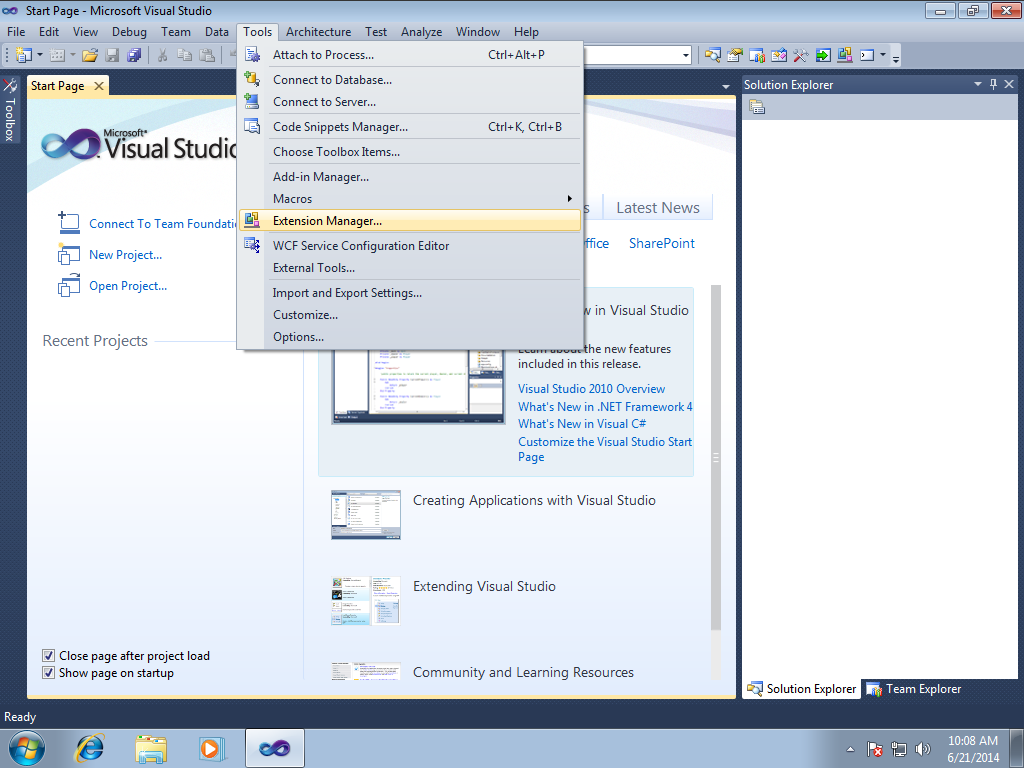
\includegraphics[width=\textwidth]{img/ankh1}
	\end{subfigure}
	\\\hfill\\
	\begin{subfigure}[t]{5in}
		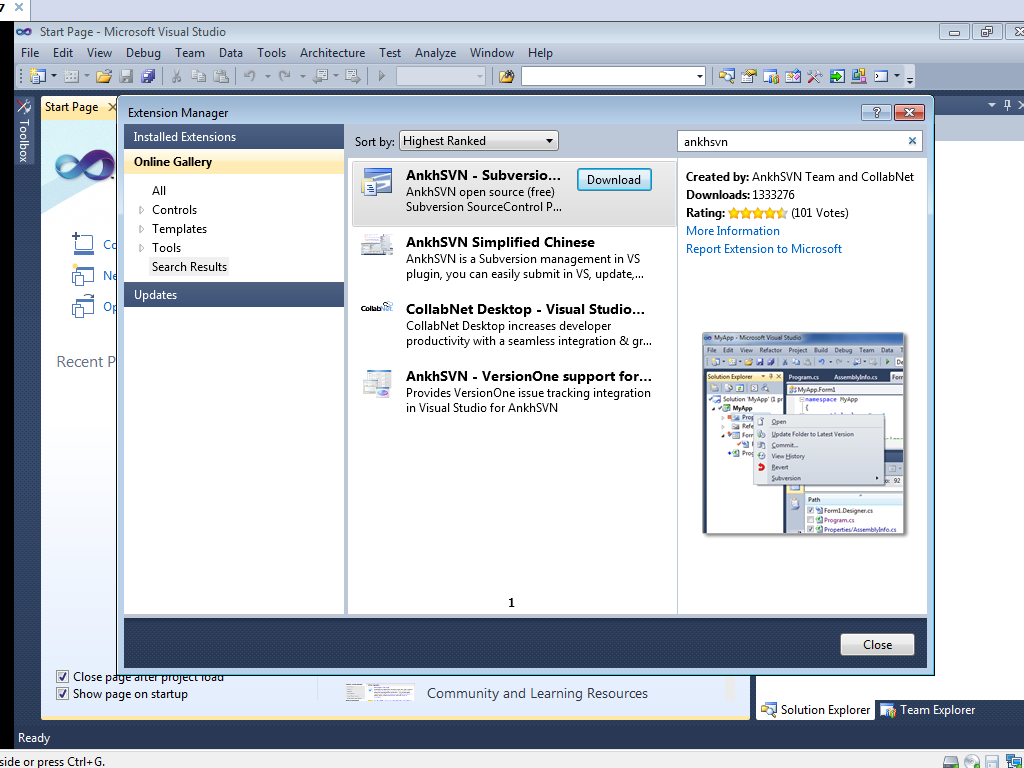
\includegraphics[width=\textwidth]{img/ankh2}
	\end{subfigure}
	\caption{Installatie van AnkhSVN}
	\label{fig:ankh1}
\end{figure}

\begin{figure}[H]
\centering
	\begin{subfigure}[t]{5in}
		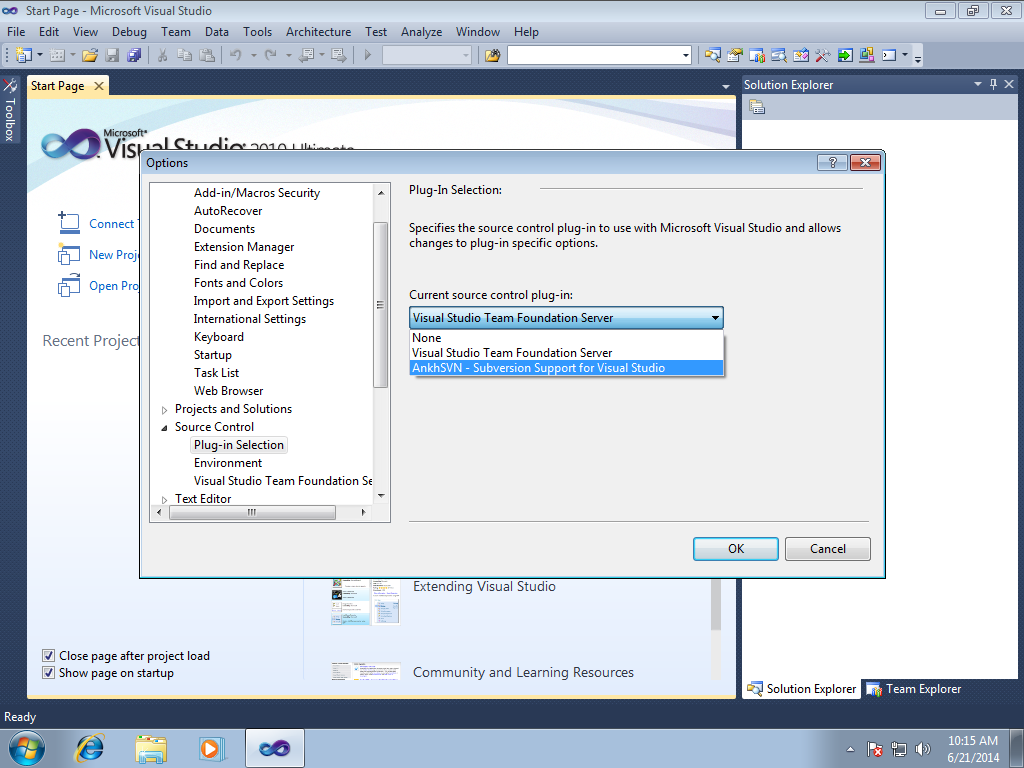
\includegraphics[width=\textwidth]{img/ankh3}
		\caption{AnkhSVN activeren}
		\label{fig:ankh3}
	\end{subfigure}
	\\\hfill\\
	\begin{subfigure}[t]{5in}
		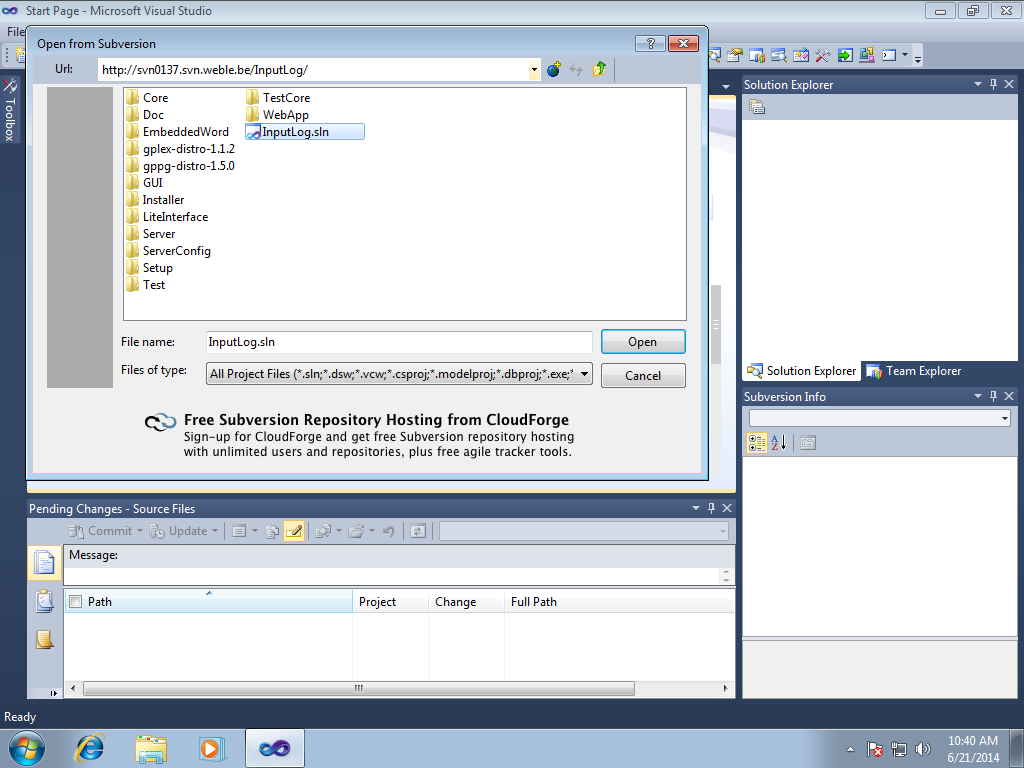
\includegraphics[width=\textwidth]{img/ankh4}
		\caption{Inputlog downloaden via AnkhSVN}
		\label{fig:ankh4}
	\end{subfigure}
\end{figure}

\subsection{Inputlog Solution}
De solution is nu zichtbaar in Visual Studio. Je krijgt vermoedelijk een error in verband met het (deprecated) Setup-project dat niet ingelezen kan worden. Dit is een InstallShield project maar wordt momenteel niet meer gebruikt en is dus ook niet belangrijk. Ook het WebApp project zal niet ingeladen kunnen worden, dit komt in de volgende sectie aan bod. De solution overview ziet er vermoedelijk uit zoals in figuur \ref{fig:solution}. De volgende stap is het ``signen'' van de verschillende projecten. Dit doe je door via rechtermuisknop op het project naar Properties te gaan. Onderaan vind je daar een tab ``Signing'', en op dat tabblad (als het project een signature heeft) een knop ``Change Password''. Hier klik je op en vervolgens typ je 3x hetzelfde wachtwoord in, terug te vinden in het document met de wachtwoorden en URLs. Figuur \ref{fig: signing} illustreert dit. Na deze stap kan je normaal gezien succesvol builden. Momenteel vereisen volgende projecten signing:

\begin{itemize}
\item EmbeddedWord
\item GUI
\item InputLog.Core
\item WebApp
\end{itemize}

\begin{figure}[H]
\centering
	\begin{subfigure}[t]{5in}
		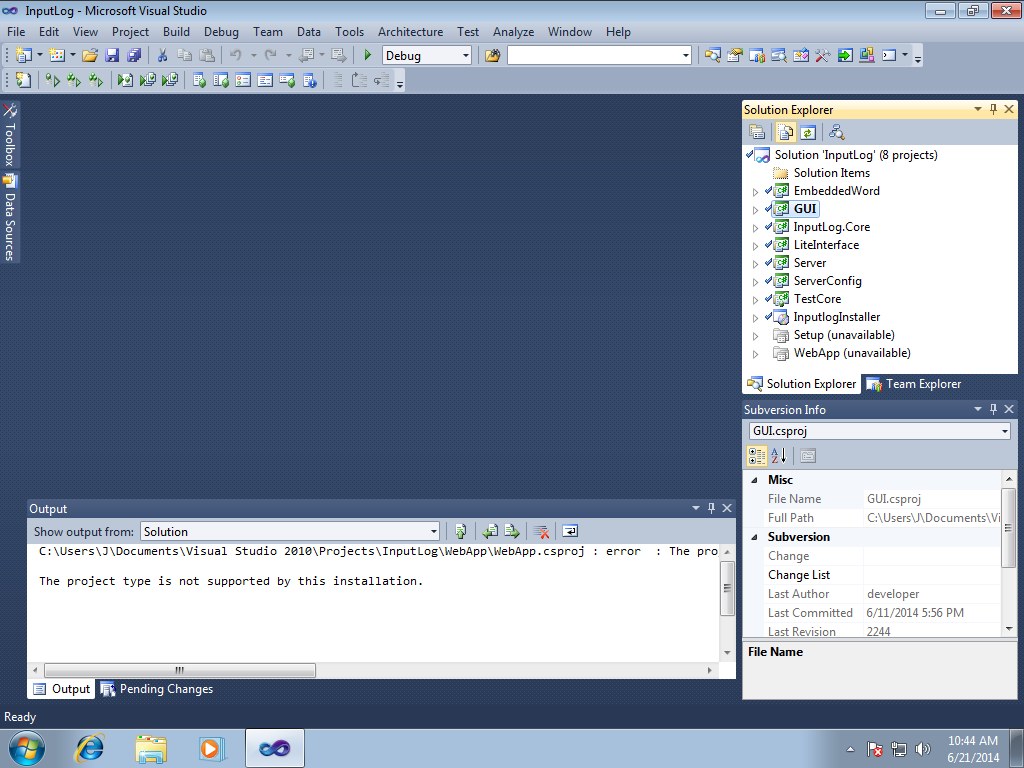
\includegraphics[width=\textwidth]{img/solution}
		\caption{Overzicht van de Inputlog Solution}
		\label{fig:solution}
	\end{subfigure}
	\\\hfill\\
	\begin{subfigure}[t]{5in}
		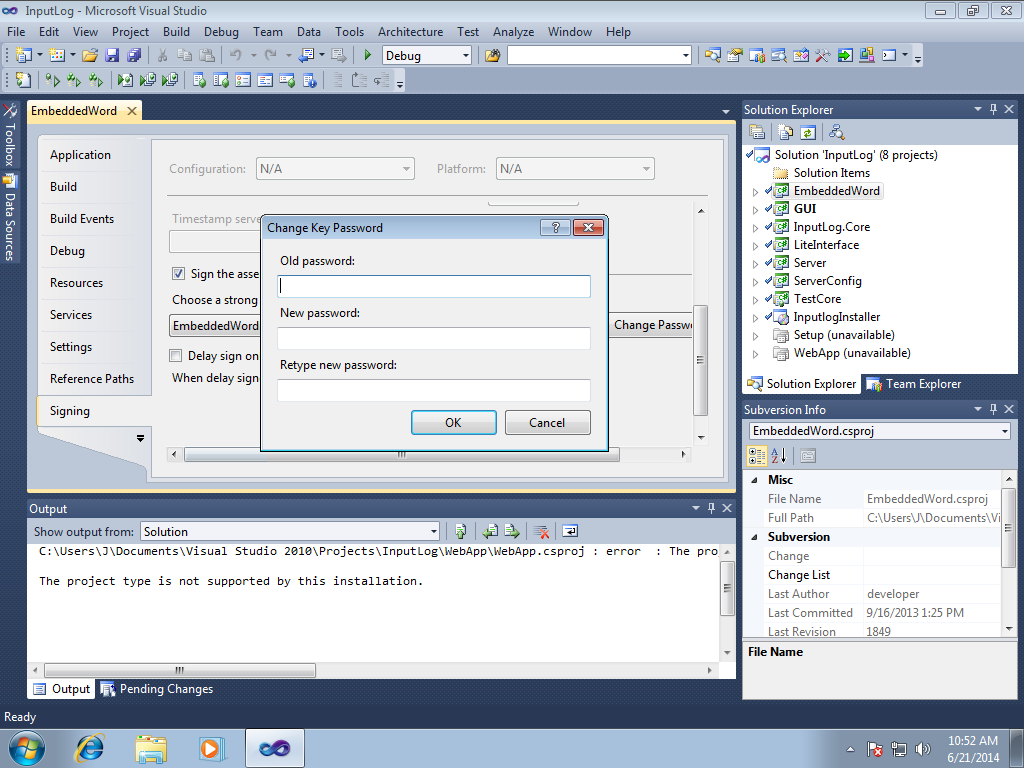
\includegraphics[width=\textwidth]{img/signing}
		\caption{Signing van de Inputlog projecten}
		\label{fig:signing}
	\end{subfigure}
\end{figure}

\subsection{WebApp}
Voor het uitvoeren van de WebApp moet eerst het ASP MVC framework versie 3 ge\"installeerd worden (\href{http://www.asp.net/mvc/mvc3}{link}). Daarnaast moet je een localhost MySQL server draaiende hebben, bijvoorbeeld via Wamp. Verder moeten er 2 MySQL adapters ge\"installeerd worden: ODBC en .NET (feel free om de WebApp zodanig aan te passen dat er slechts \'e\'en adapter vereist is \ldots). Deze adapters moeten overeen stemmen met de versies aangeduid in het bestand web.config van de WebApp (zie figuur \ref{fig:webconf}), dus ofwel moeten de vernoemde versies worden ge\"installeerd ofwel moeten de versienummers na installatie ge\"update worden. Let op: de versie van de ``UA Server'' moet niet aangepast worden. Indien hier nog problemen mee optreden heeft dit meestal met x86/x64 versie problemen te maken.

Ten slotte moet er voor Inputlog een database worden aangemaakt. Importeer in deze database het bestand ``InputlogBasis.sql'' dat je in dezelfde map als dit bestand vindt. Hierin zit de basis structuur van de database en een prefab adminaccount met gebruikersnaam \texttt{UAdmin} en wachtwoord \texttt{aaaaaa}. Zorg er tevens voor dat de MySQL inloggegevens van je server/database in het web.config bestand zijn aangepast. Hierna kan je de WebApp zonder problemen builden en starten.

\begin{figure}[H]
\centering
	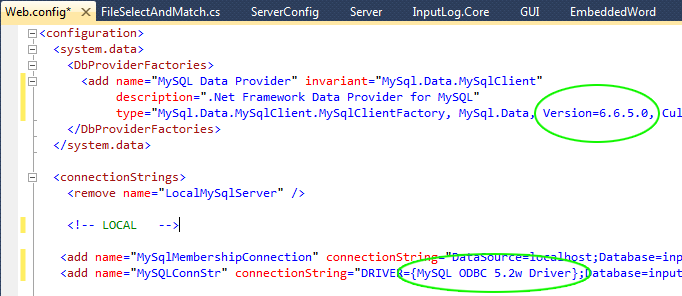
\includegraphics[width=5in]{img/webconf}
	\caption{MySQL adapter versies in de WebApp config}
	\label{fig:webconf}
\end{figure}

\newpage
\section{Project Overview}
In deze sectie worden de verschillende InputLog deelprojecten kort besproken. Figuur \ref{fig:DepGraph} toont de interne dependency graph van deze projecten. Groen aangeduid zijn de 3 kernprojecten die nodig zijn voor een ``gewone'' build. 

\begin{description}
\item[InputLog.Core:] \hfill\\ Dit project bevat alle basisfunctionaliteit die gedeeld wordt (of zou kunnen worden \ldots) door de andere projecten. Hiertoe behoren onder andere de Analyses, IO functionaliteit, de eigenlijke Logging, en een hoop diverse Utilities die hopelijk allemaal kort beschreven zijn in de InputLog Reference Guide. Ieder ander project steunt op de InputLog Core.
\item[EmbeddedWord:] \hfill\\ Een zeer vervelend lowlevel project dat de functionaliteit achter de ``Play'' tab van InputLog voorziet. Het project zelf is solide, het linken van het output OCX bestand loopt regelmatig mis om onduidelijke redenen. Best om hier niet aan te prutsen.
\item[GUI:] \hfill\\ Output project dat de normale InputLog GUI genereert. Met deze GUI lopen ook regelmatig dingen mis in verband met uitlijning van elementen, zeker in geval van resolutiewijziging of uitrekken van de GUI. Aanraken op eigen risico. Verder bevat dit project ook klasses die voor de functionaliteit achter de tabbladen zorgen, zoals de Recorder, de verschillende Analyzers en Preprocessors, \ldots Maakt voor de merging in de PreProcess tab gebruik van een ingenieus Wizard-systeem dat hopelijk beschreven is in de Reference Guide, courtesy of Tom Pauwaert.
\item[LiteInterface:] \hfill\\ WPF project voor de InputLog lite versie. De Lite versie voorziet een zo eenvoudig mogelijke interface die enkel logging ondersteunt (en backups maakt van het oorspronkelijke document). De resultante IDFX bestanden worden ge\"upload naar de Inputlog server. Het proces om een Inputlog Lite onderzoeksproject op te starten is gedefinieerd in de reference guide.
\item[WebApp:] \hfill\\ MVC ASP project dat de administratie van de Inputlog Server regelt. Accounts aanmaken, mails sturen, overzicht voor de gebruiker en tevens een administratie gedeelte voor de beheerders. Projecten worden gestart via een HTTP formulier waar gebruikers de URL niet van weten, dit formulier wordt achter de schermen door de Client ingevuld. Projecten worden dan in de database ingeschreven en de schijf geplaatst waar de Server deze verder afhandelt. Precieze gang van zaken is beschreven in de reference guide.
\item[Server:] \hfill\\ Project dat Inputlog taken afhandelt op de server, in verschillende threads. Resultaten worden op de server bewaard en opgehaald door de GUI of manueel door de gebruiker langs de WebApp.
\item[ServerConfig:] \hfill\\ Simpele administratietool voor InputLog zaken op de server. Dient met een adminaccount geconfigureerd te worden en kan vervolgens periodiek opruimen en mails versturen (scheduling door Windows).
\item[TestCore:] \hfill\\ Test framework, beschreven in sectie \ref{sec:test}.
\item[Setup:] \hfill\\ Deprecated project van de oude InstallShield installer.
\item[InputlogInstaller:] \hfill\\ Project voor de huidige installer.
\end{description}

\begin{figure}[H]
\centering
	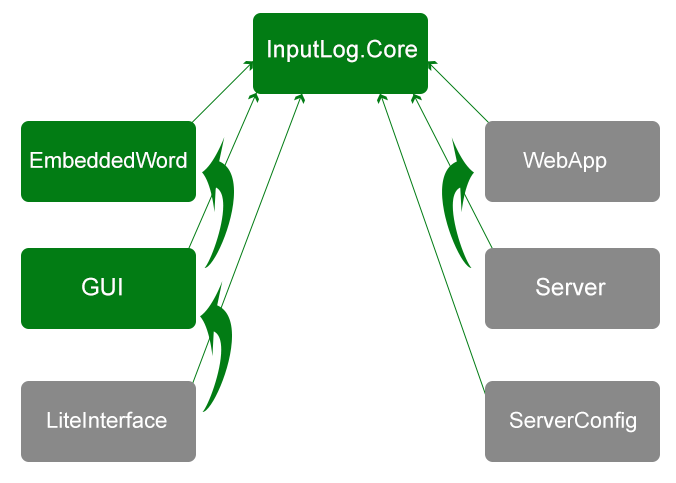
\includegraphics[width=5in]{img/DepGraph}
	\caption{Interne dependency graph van de Inputlog projecten}
	\label{fig:DepGraph}
\end{figure}

\newpage
\section{Application Flow}
\subsection{Recording}
\begin{enumerate}
\item Recorder object wordt aangemaakt, ofwel met reeds ingestelde RecordSettings ofwel met reference naar Record tab (Settings worden on demand opgehaald uit de GUI)
\item Klik ``Start Recording'', Recorder lanceert alle plugins die geselecteerd zijn (plugin selectie gebeurt via Options)
\item Klik ``Stop Recording'', IDFX wordt uitgeschreven en Analyze tab wordt geactiveerd
\end{enumerate}

\subsection{Preprocess}
\begin{enumerate}
\item Met de knop ``source files'' bovenaan worden input idfx bestanden gekozen
\item Via de radio buttons kan een preprocessor gekozen worden, deze wordt geactiveerd in preprocess.cs
\item Klik ``Process'', in preprocess.cs wordt nu een Handle\ldots() functie aangeroepen om de bestanden te verwerken:
\begin{description}
\item[Filter/Recode:] In HandleEventProcessing() worden alle geselecteerde idfx bestanden \'e\'en voor \'e\'en ingelezen en vervolgens door alle geselecteerde processors gejaagd
\item[Merging/Segmentation:] In HandleSegmentProcessing() of HandleMergeProcessing() worden alle bestanden in \'e\'en keer aan een IDFXMergingProcess of een IDFXSegmentationProcess() gegeven en gemerged dan wel gesegmenteerd terug uitgeschreven
\item[File-level:] Afhankelijk van de keuze wordt een apart venster geopend, een ConversionForm of een Merging wizard. Selectie van bestanden etc gebeurt in deze aparte vensters, allemaal terug te vinden in respectivelijk de mappen Preprocess/Conversion en Preprocess/Merge. Merging heeft hier betrekking op IDFX bestanden (verschil met PostProcess)
\end{description}
\end{enumerate}

\subsection{Analyze}
\begin{enumerate}
\item AnalysisControls worden via de ``Add'' knop geselecteerd, toegevoegd in GUI en in een lijst bewaard in Analyze.cs (verpakt in een AnalysisWrapper die de minimize en delete icoontjes voorziet)
\item AnalysisControls bieden inputs om analyses te configureren, op basis daarvan genereren ze later een Analyzer
\item Klik ``Analyze'', de AnalysisControls worden nu sequentieel overlopen
\item Per AnalysisControl worden \'e\'en voor \'e\'en alle input IDFX bestanden overlopen en geanalyzeerd (methode Analyze() in de AnalysisControl wordt opgeroepen)
\item Deze methode genereert per bestand een Analyzer die de analyse aanroept en uitschrijft (voor ServerAnalysis worden alle IDFX's geserializeerd en bijgehouden, en achteraf in \'e\'en keer verzonden naar de server)
\item De eigenlijke analyses bevinden zich in Core/Analyses, ieder met een eigen map en opgedeeld in een Analysis (berekening), AnalysisSummary (resultaten) en AnalysisWriter (schrijft Summary naar file)
\item GUI wordt ge\"update met de Open File link in de analysiswrapper (link naar de output van het laatst verwerkte IDFX bestand)
\end{enumerate}

\subsection{Postprocess}
\begin{enumerate}
\item Klik op ``merge consecutively logged \ldots'' en de wizard uit Tabs/Postprocess/WizardPages wordt gestart (merging van analyse outputs, niet te verwarren met merging in Preprocess stap)
\item De eigenlijke merging klasses bevinden zich in Core/Merging/Analyses, er wordt een Horizontale of Verticale merger aangemaakt
\item De merger gebruikt de functionaliteit uit IO/AnalysisXML om de analyses in te lezen in een dictionary, die dan verticaal of horizontaal wordt samengevoegd (meer info in de reference guide)
\end{enumerate}

\subsection{Play}
\begin{enumerate}
\item \ldots
\end{enumerate}

\newpage
\section{Test Framework}\label{sec:test}
De Inputlog tests maken gebruik van NUnit. Via de extension manager kan Visual NUnit ge\"installeerd worden op dezelfde wijze als AnkhSVN. Na installatie kan je via View $\Rightarrow$ Other windows $\Rightarrow$ Visual NUnit de interface oproepen. Hier selecteer je bovenaan het TestCore project, na enkele seconden wachten worden dan de beschikbare tests getoond. Via Namespace en Fixture kan je verder refinen richting 1 bepaalde testklasse, zoals in figuur \ref{fig:nunit}.

Om analyses te testen wordt gebruik gemaakt van de AnalyzerSimulator. Deze neemt een reeks input idfxen en een outputdirectory als initialisatie. Vervolgens kan de functie Run() aangeroepen worden die een ge\"initializeerd Analyzer object als argument heeft. De AnalyserSimulator roept vervolgens alle functies van de Analyser aan die de AnalysisControl normaal zou aanroepen. Als resultaat wordt er een analyse XML uitgeschreven die vergeleken kan worden met een verwachte output. Uiteraard kunnen er dummy wrappers rond de Analyzers geschreven worden om bepaalde functionaliteit uit te schakelen etc.

Tests halen hun input idfx bestanden uit de map InputData, en schrijven uit naar ActualOutput. Verwachte output wordt in ExpectedOutput opgeslagen. Zorg er zeker voor dat ``Copy to output directory'' is ingesteld voor ieder bestand (zie properties). Klasse TestUtils bevat enkele functies om gelijkheden na te gaan, bijvoorbeeld van 2 bestanden (niet te verwarren met de map TestUtil, die tests van utility klasses bevat).

Houd er bij het uitvoeren van alle tests rekening mee dat sommigen (voornamelijk Revision) tamelijk veel tijd in beslag kunnen nemen \ldots
\begin{figure}[H]
\centering
	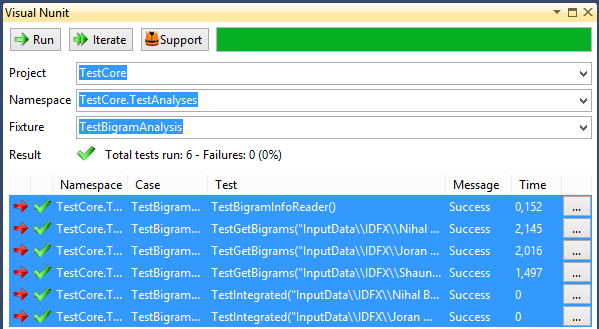
\includegraphics[width=5in]{img/nunit}
	\caption{Tests runnen met Visual NUnit}
	\label{fig:nunit}
\end{figure}
\end{document}